\documentclass[11pt]{article}
\usepackage[utf8]{inputenc}
\usepackage{amsmath,amsthm,amsfonts,amssymb,amscd}
\usepackage{multirow,booktabs}
\usepackage{enumitem}
\usepackage{fancyhdr}
\usepackage{mathrsfs}
\usepackage{wrapfig}
\usepackage{setspace}
\usepackage{calc}
\usepackage{multicol}
\usepackage{cancel}
\usepackage[retainorgcmds]{IEEEtrantools}
\usepackage{framed}
\usepackage[most]{tcolorbox}
\usepackage{tikz}
\usepackage{geometry}
\geometry{
	a4paper,
	total={170mm,257mm},
	left=20mm,
	top=20mm,
}
\title{Vectors}
\author{Aaron G.K.}
\begin{document}
	\maketitle
	Vectors are essential to physics and engineering. Many fundamental physical quantities are vectors, including displacement, velocity, force, and electric and magnetic vector fields. Scalar products of vectors define other fundamental scalar physical quantities, such as energy. Vector products of vectors define still other fundamental vector physical quantities, such as torque and angular momentum. In other words, vectors are a component part of physics in much the same way as sentences are a component part of literature.
	\subsection*{Scalars and Vectors}
    Many physical quantities can be specified completely by giving a single number and the appropriate unit. For example, “a class period lasts 50 min” or “the gas tank in my car holds 65 L” or “the distance between two posts is 100 m.” A physical quantity that can be specified completely in this manner is called a scalar quantity. Scalar is a synonym of “number.” Time, mass, distance, length, volume, temperature, and energy are examples of scalar quantities.
    \\ \\
    Some other physical quantities, however, cannot be described completely by just a single number of physical units - they may need a direction attached to the scalar to give it the full meaning. Physical quantities specified completely by giving a number of units (magnitude) and a direction are called vector quantities. 
    \subsection*{Representation of Vectors}
    \begin{center}
    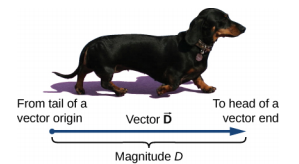
\includegraphics[scale=0.5]{dog.png}	
    \end{center}
    We draw a vector from the initial point or origin (called the \textbf{tail}) to the end or terminal point (called the \textbf{head}), marked by an arrowhead. Magnitude is the length of a vector and is \textbf{always a positive }scalar quantity. \\ \\
    To see how vectors work, let's take a simple displacement vector shown in the figure below.
    \begin{center}
    	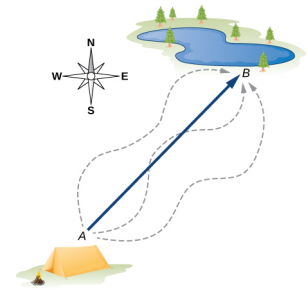
\includegraphics[scale=0.4]{disp.png}
    \end{center}
    The displacement vector from point A to point B is indicated by an arrow with origin at point A and end at point B. The displacement is the same for any of the actual paths (dashed curves) that may be taken between points A and B. \\ \\
    Two vectors that have identical directions are said to be parallel vectors—meaning, they are parallel to each other. Two parallel vectors $\vec{A}$ and $\vec{B}$ are equal, denoted by $\vec{A}=\vec{B}$, if and only if they have equal magnitudes $\vec{A}=\vec{B}$. Two vectors with directions perpendicular to each other are said to be orthogonal/perpendicular vectors. 
    \begin{center}
    	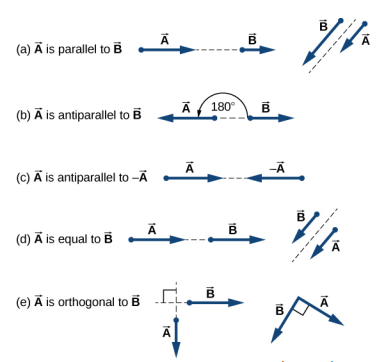
\includegraphics[scale=0.6]{vectors.png}
    \end{center}
    .
\end{document}	